% Western University Thesis Template
% By: Dr. Zhengyuan Deng, 2024

\documentclass[12pt,
              %  draft, % speed up compilation without images
               oneside,
               letterpaper]{report}
% ---------------------------------------
% fonts and encoding
\usepackage[utf8]{inputenc} % Uses the utf8 input encoding
\usepackage[T1]{fontenc} 
% \usepackage{mathpple} % Palatino
% \usepackage{mathpazo} % Palatino
% font - Times New Roman
\usepackage[spacing=.3em,
            stretch=.2em,
            shrink=.1em]{newtxtext}
\usepackage{newtxmath}
% ---------------------------------------
% Citation, reference, and bibliography
\usepackage[style=apa,
            backend=biber,
            uniquename=false,
            uniquelist=false
            ]{biblatex}
\addbibresource{westernthesis.bib} % Imports bibliography file
% hyper reference definition
\usepackage[dvipsnames]{xcolor}
% \definecolor{myColor}{RGB}{88, 44, 131} % purple
\definecolor{myColor}{rgb}{0, 0, 0} % black
\usepackage{hyperref}
\hypersetup{colorlinks = true, 
            urlcolor   = myColor, 
            linkcolor  = myColor, 
            citecolor  = myColor 
            }
% auto reference
\def\equationautorefname~#1\null{Equation~(#1)\null}
\def\chapterautorefname{Chapter}
\def\sectionautorefname{Section}
\def\subsectionautorefname{Section}
\usepackage[byname]{smartref} % Smart cross-referencing
% ---------------------------------------
% math environment
% \usepackage{amssymb} % For math symbols
\usepackage{amsmath} % For typesetting math
\usepackage{mathtools}
\usepackage[group-separator={,},
            group-digits=integer]{siunitx} % SI unit
\usepackage[version=4]{mhchem} % chemical
\usepackage{bm} % bold and italia
\usepackage{cancel} % \cancelto
\usepackage{esint} % kinds of integral signs
\usepackage{physics} % for physics
\sisetup{
  % range-phrase = \text{-}, 
  range-units = single,
  table-alignment-mode = format
}
\usepackage{xparse} % for physics
\usepackage{mathrsfs} % \mathscr
\usepackage{setspace} % line spacing
\AtBeginDocument{\RenewCommandCopy\qty\SI} % avoid conflict of \qty btw siunitx & physics

% ---------------------------------------
% table environments
\usepackage{longtable} % Long tables
\usepackage{rotating} % Rotate the figure or table
\usepackage{booktabs}
\usepackage{array} 
% \usepackage{tablefootnote}
\usepackage{multirow} % Multirow cells in tables
\usepackage{enumitem} % Customizing lists

% ---------------------------------------
% figure environments
\usepackage{graphicx}
\usepackage{caption}
\usepackage{subcaption}
% \usepackage[nofiglist, figuresonly]{endfloat} % put figures at end of chapter

% ---------------------------------------
% code environments
\usepackage{listings} 
\definecolor{codegreen}{rgb}{0,0.6,0}
\definecolor{codegray}{rgb}{0.5,0.5,0.5}
\definecolor{codepurple}{rgb}{0.58,0,0.82}
\definecolor{backcolour}{rgb}{0.95,0.95,0.92}

\lstdefinestyle{mystyle}{
    % backgroundcolor=\color{backcolour},   
    commentstyle=\color{codegreen},
    keywordstyle=\color{magenta},
    numberstyle=\tiny\color{codegray},
    stringstyle=\color{codepurple},
    basicstyle=\scriptsize\ttfamily,
    breakatwhitespace=false,         
    breaklines=true,                 
    captionpos=b,                    
    keepspaces=true,                 
    numbers=left,                    
    numbersep=5pt,                  
    showspaces=false,                
    showstringspaces=false,
    showtabs=false,                  
    tabsize=2
}

\lstset{style=mystyle}

% ---------------------------------------
\newcommand{\newcheckmark}{\raisebox{0.6ex}{\scalebox{0.7}{$\sqrt{}$}}}
\newcommand{\newcrossmark}{\scalebox{0.85}[1]{$\times$}}

% ---------------------------------------
% line space setting
% To produce output with the desired line spacing, the argument of
% \spacing should be multiplied by 5/6 = 0.8333, so that 1.5 spaced
% corresponds to \spacing{1.25} and double spaced is \spacing{1.66}.
\def\normalspacing{1.25} % default line spacing
\spacing{1.25} % 1.5 spacing

% ---------------------------------------
% page margin setting
\usepackage{geometry}
\geometry{left=1.5in, right=1in, top=1.2in, bottom=1in}
\usepackage{fancyhdr}

% ---------------------------------------
% chapter title setting
\usepackage{titlesec}
\titleformat{\chapter}[display]{\onehalfspacing\normalfont\LARGE\bfseries}{\chaptertitlename\ \thechapter}{10pt}{\LARGE}
\titlespacing*{\chapter}{0pt}{30pt}{30pt}
\titlespacing*{\section}{0pt}{10pt}{0pt}
\titlespacing*{\subsection}{0pt}{10pt}{0pt}
\titlespacing*{\subsubsection}{0pt}{0pt}{0pt}
\titlespacing*{\paragraph}{0pt}{0pt}{15pt}

\setcounter{tocdepth}{3} % Number the subsubsection 
\usepackage{mfirstuc} % Capitalize the first letter of a word

% ---------------------------------------
% Page numbering setting
\makeatletter
\numberwithin{figure}{chapter}

\newenvironment{preliminary}%
{
  \pagestyle{plain}\pagenumbering{roman}
} {
  \pagenumbering{arabic}
}

\addtoreflist{chapter}

% ---------------------------------------
% theorem environments
\newtheorem{theorem}{Theorem}[section]
\newtheorem{lemma}[theorem]{Lemma}
\newtheorem{proposition}[theorem]{Proposition}
\newtheorem{corollary}[theorem]{Corollary}

% ---------------------------------------
% Appendices environment
\usepackage[titletoc]{appendix} 
% \usepackage{appendix} 
\usepackage{tocloft} % Customizing the table of contents
\setlength{\cftchapnumwidth}{0pt}
\renewcommand{\cftchappresnum}{\chaptername\ }
\renewcommand{\cftchapaftersnum}{}
\renewcommand{\cftchapaftersnumb}{\newline}
\renewcommand{\cftchapleader}{\cftdotfill{\cftdotsep}}
% ---------------------------------------
% appendices setting
\newcommand{\listappendixname}{List of Appendices}
\newlistof{myappendices}{app}{\listappendixname}
\newcommand{\myappendices}[1]{%
\addcontentsline{app}{myappendices}{#1}\par}

% ---------------------------------------
% Titles of TOC setups
% \renewcommand{\contentsname}{Table of Contents} % Table of contents title
\renewcommand{\contentsname}{\hfill\bfseries\LARGE Table of Contents\hfill} 
\renewcommand{\cftaftertoctitle}{\hfill}
\renewcommand{\listtablename}{\hfill\bfseries\LARGE List of Tables} 
\renewcommand{\cftafterlottitle}{\hfill}
\renewcommand{\listfigurename}{\hfill\bfseries\LARGE List of Figures}
\renewcommand{\cftafterloftitle}{\hfill}
% \renewcommand{\listappendixname}{\hfill\bfseries\Large List of Appendices}
\renewcommand{\listappendixname}{\LARGE\begin{center}\textbf{List of Appendices}\end{center}}
\renewcommand{\cftafterloftitle}{\hfill}

% ---------------------------------------
% nomenclature setting
\usepackage{nomencl}
\makenomenclature
% This code creates the groups
\usepackage{etoolbox}
\renewcommand\nomgroup[1]{%
  \item[\bfseries
  \ifstrequal{#1}{S}{Symbols}{ % for symbols
  \ifstrequal{#1}{B}{Subscripts}{ % for subscripts
  \ifstrequal{#1}{G}{Symbols (greek letters and others)}{ % for greek letters
  \ifstrequal{#1}{A}{Abbreviations}{}}}} % for abbreviations
]}
\renewcommand{\nomname}{\LARGE\begin{center}\textbf{List of Abbreviations, Symbols, and Nomenclature}\end{center}}%
% ---------------------------------------
% nomenclature setting of the style and layout
\usepackage{multicol}
\nomlabelwidth=7.5mm % width of the nomenclature label
\setlength{\columnsep}{10mm} % column separation distance
\newcommand{\nomunit}[1]{ % 
  \renewcommand{\nomentryend}{\hspace*{\fill}#1}
} % nomenclature unit
\renewcommand{\nompreamble}{\begin{multicols}{2}} % two columns
\renewcommand{\nompostamble}{\end{multicols}}

% ---------------------------------------
% ---------------------------------------
% other settings
\usepackage{silence} % silence warning when compiling
\WarningFilter{fancyhdr}{\headheight is too small}

% ------------------------------------------------------------------------------
% 
%                            DOCUMENT STARTS HERE
% 
% ------------------------------------------------------------------------------

\begin{document}
% ------------------------------------------------------------------------------
% Preliminary Parts, includes: 
% Abstract
% Summary for Lay Audience
% Co-Authorship Statement
% Acknowledgements
% Table of Contents
% List of Figures
% List of Tables
% List of Appendices
% List of Abbreviations, Symbols, and Nomenclature
% They are edited in the corresponding files in the folder "preliminaries".
% ---------------------------------------
\begin{preliminary}
% ---------------------------------------------------
%  Abstract
% ---------------------------------------------------
\addcontentsline{toc}{chapter}{Abstract}
\LARGE\begin{center}\textbf{Abstract}\end{center}\normalsize
\setcounter{page}{2}
% \LARGE\textbf{Abstract}\normalsize
\vspace{30pt}
% ---------------------------------------------------
%%  ***  Put your Abstract here.   ***
%% (350 words for Ph.D.)
% --------------------------------------------------
This is your silly abstract here.

% --------------------------------------------------
% \vspace{20pt}
\vfill
\noindent\textbf{Keywords:} Silly, keywords 
% ---------------------------------------------------
\newpage
% ---------------------------------------------------
%  Summary for Lay Audience
% ---------------------------------------------------
\phantomsection
\addcontentsline{toc}{chapter}{Summary for Lay Audience}
\LARGE\begin{center}\textbf{Summary for Lay Audience}\end{center}\normalsize
% \LARGE\textbf{Summary for Lay Audience}\normalsize
\vspace{30pt}
% ---------------------------------------------------
% From Thesis Regulation Guide section 3.1.8:
% The summary for lay audience is a brief (maximum 350 words) and accessible summary of a research project that is used to explain complex ideas, technical writing and scientific terms to people who do not have prior knowledge of the subject. While your abstract is designed with your subject peers in mind, the Summary for Lay Audience communicates the importance, impact, and content of your thesis to a broader audience.
%%  ***  Put your Summary for Lay Audience   ***
Here is your Summary for Lay Audience.

% ---------------------------------------------------
\newpage
% ---------------------------------------------------
%  Co-Authorship Statement
% ---------------------------------------------------
\phantomsection
\addcontentsline{toc}{chapter}{Co-Authorship Statement}
\LARGE\begin{center}\textbf{Co-Authorship Statement}\end{center}\normalsize
% \LARGE\textbf{Co-Authorship Statement}\normalsize
\vspace{30pt}
% ---------------------------------------------------
%%  ***  Put your Co-Authorship Statement here.   ***
Your Co-Authorship Statement here.

% ---------------------------------------------------
\newpage
% ---------------------------------------------------
%  Acknowledgements
% ---------------------------------------------------
\phantomsection
\addcontentsline{toc}{chapter}{Acknowledgements}
\LARGE\begin{center}\textbf{Acknowledgements}\end{center}\normalsize
% \LARGE\textbf{Acknowledgements}\normalsize
\vspace{30pt}
% ---------------------------------------------------
%%  ***  Put your Acknowledgements here.   ***
Here is your acknowledgements.

First and foremost, I would like to express my deepest gratitude to my main supervisor...
% ---------------------------------------------------
\newpage
% ---------------------------------------------------
%  Table of Contents
% ---------------------------------------------------
\phantomsection
\addcontentsline{toc}{chapter}{Table of Contents}
\tableofcontents
\newpage
% ---------------------------------------------------
\phantomsection
\addcontentsline{toc}{chapter}{List of Figures}
\listoffigures
\newpage
% ---------------------------------------------------
\phantomsection
\addcontentsline{toc}{chapter}{List of Tables}
\listoftables
\newpage
% ---------------------------------------------------
% \phantomsection
% \addcontentsline{toc}{chapter}{List of Appendices}
% \listofmyappendices
% \newpage
% ---------------------------------------------------
\phantomsection
\addcontentsline{toc}{chapter}{List of Abbreviations, Symbols, and Nomenclature}
\nomenclature[S]{$H$}{Height, $\si{\m}$}
\nomenclature[S]{$A$}{Area, $\si{\m^2}$}
\nomenclature[S]{$D$}{Diameter, $\si{\m}$}
% 
% 
% 
% 
% 
% 
% 
\nomenclature[G]{$\Gamma$}{Mass diffusivity, $\si{\kg/\m/\s}$}
\nomenclature[G]{$\rho$}{Density, $\si{\kg/\m^3}$}
\nomenclature[G]{$\mu$}{Viscosity, $\si{\kg/\m/\s}$}
% 
% 
% 
% 
% 
% 
% 
\nomenclature[B]{g}{Gas phase}
\nomenclature[B]{s}{Solids phase}
% 
% 
% 
% 
% 
% 
% 
\nomenclature[A]{CFB}{Circulating fluidized bed}
\nomenclature[A]{CFD}{Computational fluid dynamics}
\nomenclature[A]{PDF}{Probability distribution function}
\nomenclature[A]{CDF}{Cumulative distribution function}
\nomenclature[A]{FCC}{Fluid catalytic cracking}
\printnomenclature
% ---------------------------------------------------
\newpage
% ---------------------------------------------------
\end{preliminary}
% ---------------------------------------
% End of the preliminary sections
% ------------------------------------------------------------------------------
% Set spacing of texts and equations for the main body of the thesis.
% ---------------------------------------
\setlength\parindent{2em} % paragraph indent
\setlength{\parskip}{12pt} % paragraph spacing
\setlength\bibitemsep{5pt} % bibliography spacing
\setlength\jot{18pt} % equation spacing
% \spacing{0.8333} % single spacing
% \spacing{1.25} % 1.5 spacing
\spacing{1.66} % double spacing
% Set header and footer 
\setlength{\headheight}{10pt} % space of header
% \setlength{\headheight}{0pt} % space of header
\pagestyle{fancy} % fancy page style
\fancyhead{} % no header
% \fancyfoot{} % no footer
\renewcommand{\headrulewidth}{0pt} % no header rule
\raggedbottom % bottom of page is ragged
% ---------------------------------------
% End of the main body settings.
% ------------------------------------------------------------------------------
% Main body of the thesis starts here.
% ------------------------------------------------------------------------------
% Include the chapters.
% ---------------------------------------
\chapter{Introduction}
\label{chap: intro}
\fancyhead[R]{CHAPTER \thechapter. \uppercase{
    Introduction
    }}
% \fancyhead[R]{\rightmark}

\begin{refsection}
% -------------------------------------------------------
%                    BEGIN MAIN TEXT
% -------------------------------------------------------

Here is your first chapter: Introduction.

\section{Background}
Your background \autocite{deng2017volumetric}.
% -------------------------------------------------------

\section{Research objectives}
The overall objective is ...


\section{Thesis structure}
This thesis follows the integrated-article format as outlined in the thesis guide of Western University. The thesis is organized as follows:

% -------------------------------------------------------
%                    END MAIN TEXT
% -------------------------------------------------------
\pagebreak
\addcontentsline{toc}{section}{References}

\begin{spacing}{1.1}
    \printbibliography[heading=subbibliography]
\end{spacing}
\end{refsection}
\chapter{Main Chapter 1}
\label{chap: reactive transport model}
\fancyhead[R]{\uppercase{Chapter \thechapter. 
    Main Chapter 1
    }}
% \fancyhead[RE]{\rightmark}
% \fancyhead[LE, RO]{\thepage}
\begin{refsection}
% \linenumbers
\normalsize
% -------------------------------------------------------
%                    BEGIN MAIN TEXT
% -------------------------------------------------------

\section{Introduction}

This chapter comprises four parts. 

\section{Equation}
\label{sec:chap1: equation}
\subsection{Equation Example}
The equation example can be described as follows: 
\begin{equation}
    \pdv{t} \left( \varepsilon_{\mathrm{g}}\,\rho_{\mathrm{g}}\,Y_{\mathrm{g}}^{\ce{O3}} \right)
    + 
    \dots
    \label{eqn:chap1: equation example}
\end{equation}


\section{Figure}
\label{sec:chap1: Figure}
% figure: geometry and mesh of micro-reactor
\begin{figure}[!htbp]
    \centering
    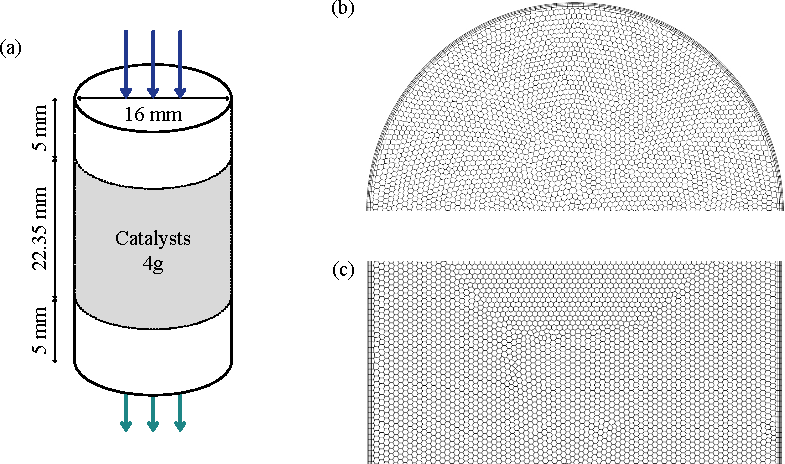
\includegraphics[width=.85\textwidth]{fig/chap_RxnMod-mesh_fixed_bed.pdf}
    \caption{Computational domain and mesh of the micro fixed-bed reactor}
    \label{fig:Chap1: mesh of micro-reactor}
\end{figure}

\autoref{fig:Chap1: mesh of micro-reactor} shows ...

\section{Table}
\label{sec:chap1: Table}

\autoref{tab:Chap1: Comparison} shows ... \autocite{liujs2016, wang2014catalytic}. 

\begin{table}[!h]
    \centering
    \vspace{10pt}
    \caption{Comparison of numerical results with experimental data}
    \begin{tabular}{cccccccc}
        \toprule
        Case & $C_{\mathrm{g,in}}^{\ce{O3}}$ & Packed $\varepsilon_{\mathrm{s}}$ & $U_{\mathrm{g}}$ & $k_\mathrm{r}$ & $C_{\mathrm{g,out}}^{\ce{O3}}$ & $ C_{\mathrm{g,out}}^{\ce{O3}}/C_{\mathrm{g,in}}^{\ce{O3}}$ & APE \\ 
        \midrule
        Unit & \si{ppmv} & - & \si{\m/\s} & \si{\per\s} & \si{ppmv} & - & \si{\percent} \\
        \midrule
        Exp. 1 $^{*}$ & 115.1 & 0.5 & 0.1124 & 4.12 & 50.70 & \num{0.44000} & - \\
        Num. 1 & 115.1 & 0.5 & 0.1124 & 4.12 & 50.84 & \num{0.44170} & 0.39 \\
        Exp. 2 $^{**}$ & 100.0 & 0.5 & 0.57 & 49.12 & 9.054 & \num{0.09054} & - \\
        Num. 2 & 100.0 & 0.5 & 0.57 & 49.12 & 9.049 & \num{0.09049} & 0.06 \\
        \bottomrule \\[-10pt]
        \multicolumn{8}{l}{\footnotesize{
            $^*$ Data from the work of \textcite{liujs2016}.}} \\
        \multicolumn{8}{l}{\footnotesize{
            $^{**}$ Data from the work of \textcite{wang2014catalytic}.}} 
    \end{tabular}
    \label{tab:Chap1: Comparison}
\end{table}

\section{Conclusions}
The present study involved 

% \processdelayedfloats % put figures here
% -------------------------------------------------------
%                    END MAIN TEXT
% -------------------------------------------------------
\pagebreak
\addcontentsline{toc}{section}{References}

\begin{spacing}{1.1}
    \printbibliography[heading=subbibliography]
\end{spacing}
\end{refsection}
% \include{chapters/chapter_2.tex}
\chapter{Conclusions and Recommendations}
\label{chap: conclustion}
\fancyhead[R]{CHAPTER \thechapter. \uppercase{
    Conclusions and Recommendations
    }}
% \fancyhead[RE]{\rightmark}
% \fancyhead[LE, RO]{\thepage}
\begin{refsection}

\section{Thesis summary and conclusions}

This thesis work comprehensively investigates ...

\autoref{fig:conclusion: reaction in gs system} depicts ...
\begin{figure}[htp]
    \vspace{10pt}
    \centering
    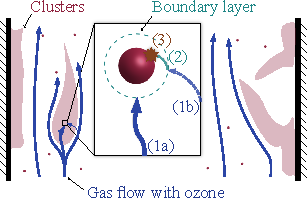
\includegraphics[width=0.45\textwidth]{fig/reaction_in_gs_system.pdf}
    \caption{Caption...}
    \label{fig:conclusion: reaction in gs system}
\end{figure}


\section{Limitations and recommendations}

Limitations ...


\pagebreak
\addcontentsline{toc}{section}{References}
\begin{singlespacing}
\printbibliography[heading=subbibliography]
\end{singlespacing}

\end{refsection}
% ---------------------------------------
% End of the chapters.
% ---------------------------------------
% Include the appendices.
% ---------------------------------------
\begin{appendices}
  \chapter{Your appendix}
\label{appendix: codes}
\fancyhead{} % clean headers
\fancyhead[R]{APPENDIX \thechapter. \uppercase{
    your appendix
    }}
\begin{refsection}
% -------------------------------------------------------
%                    BEGIN MAIN TEXT
% -------------------------------------------------------


This is your appendix \autocite{deng2017volumetric}.


\pagebreak
\addcontentsline{toc}{section}{References}

\begin{singlespacing}
\printbibliography[heading=subbibliography]
\end{singlespacing}

\end{refsection}
\end{appendices}
% ---------------------------------------
% End of the appendices.
% ---------------------------------------
% CV
% ---------------------------------------
\addcontentsline{toc}{chapter}{Curriculum Vitae}
\fancyhead{} % no header
\chapter*{Curriculum Vitae}
\begin{refsection}
\nocite{deng2017volumetric}

\begin{table}[!h]
\begin{tabular}{ll}
\textbf{Name:} & firstname lastname\\\\
\textbf{Post-Secondary} & Department of Chemical \& Biochemical Engineering\\
\textbf{Education and}& The University of Western Ontario\\
\textbf{Degrees:}& London, Ontario, Canada\\
& 2018 - present \quad Ph. D. candidate\\
\\
& School of XXX \\
& XXX \\
& Wuhan, Hubei, China\\
& 2012 - 2016 \quad B. Eng.\\
\\
\textbf{Honours and}& XXXX, 2016 \\
\textbf{Awards:} & XXXXX\\
& \\
& National Scholarship, 2015\\
& Ministry of Education of the People's Republic of China\\
& \\
\textbf{Related }& Research and Teaching Assistant, 2019 - 2023\\
\textbf{Experience:}& The University of Western Ontario, London, Ontario\\
& \\
& Visiting Student, 2021 \\
& Shanghai Jiao Tong University, Shanghai, China\\
\end{tabular}
\end{table}

\subsubsection*{Publications:}
\begin{singlespacing}
    \printbibliography[heading=none]
\end{singlespacing}
\end{refsection}
% ---------------------------------------
% End of the CV.
% ---------------------------------------
\end{document}
% ------------------------------------------------------------------------------
%
%                            DOCUMENT ENDS HERE
%
% ------------------------------------------------------------------------------
